\section{Justering ift. matematisk model af PTS}
%Bestemmelsen tager udgangspunkt i en analytisk fremgangsmåde ved brug af \emph{pidtool()}
% og Simulink simuleringen\footnote{Findes på CDROM.} af PTS. "Start" koefficienterne, angivet i 

Justeringen af PI-koefficienterne ift. den matematiske model sker ved "trial \& error" metoden. 
I praksis udføres det ved brug af Matlabs grafiske "trial \& error" redskab \emph{pidtool()} og ved at kigge 
på en 1-radian steprespons. 
De bedste koefficienterne findes i første omgang til at være som i tabel \ref{tb:PID_test14}. 
\todo[inline, author=Michael]{Hvad får vi ud af at kigge på 1 radian step? Det fremgår ikke særlig klart. Måske kunne vi starte med Ziegler Nicholls istedet.}
\begin{figure}[h!]
\centering
\begin{tabu}{l|[1.25pt]c|c|c}
      & \(K_P\) & \(K_I\) & \(K_D\)\\\tabucline[1.25pt]{-}
Tilt  & 38,5 & 20 & -\\\hline%0,248960\\\hline
Pan   & 27 &  6,83 & -
\end{tabu}
\captionsetup{type=table}
\caption[Regulator koefficienter]{Koefficienter fundet ud fra den matematiske model.}
\label{tb:PID_test14} 
\end{figure}

Denne PI-regulator afprøves på PTS med henblik på at se den reelle performance 
af systemet. Fejlen fra den ønskede position plottes i figur \ref{fig:PID_test14_plot}.
\begin{figure}[h!]
\centering
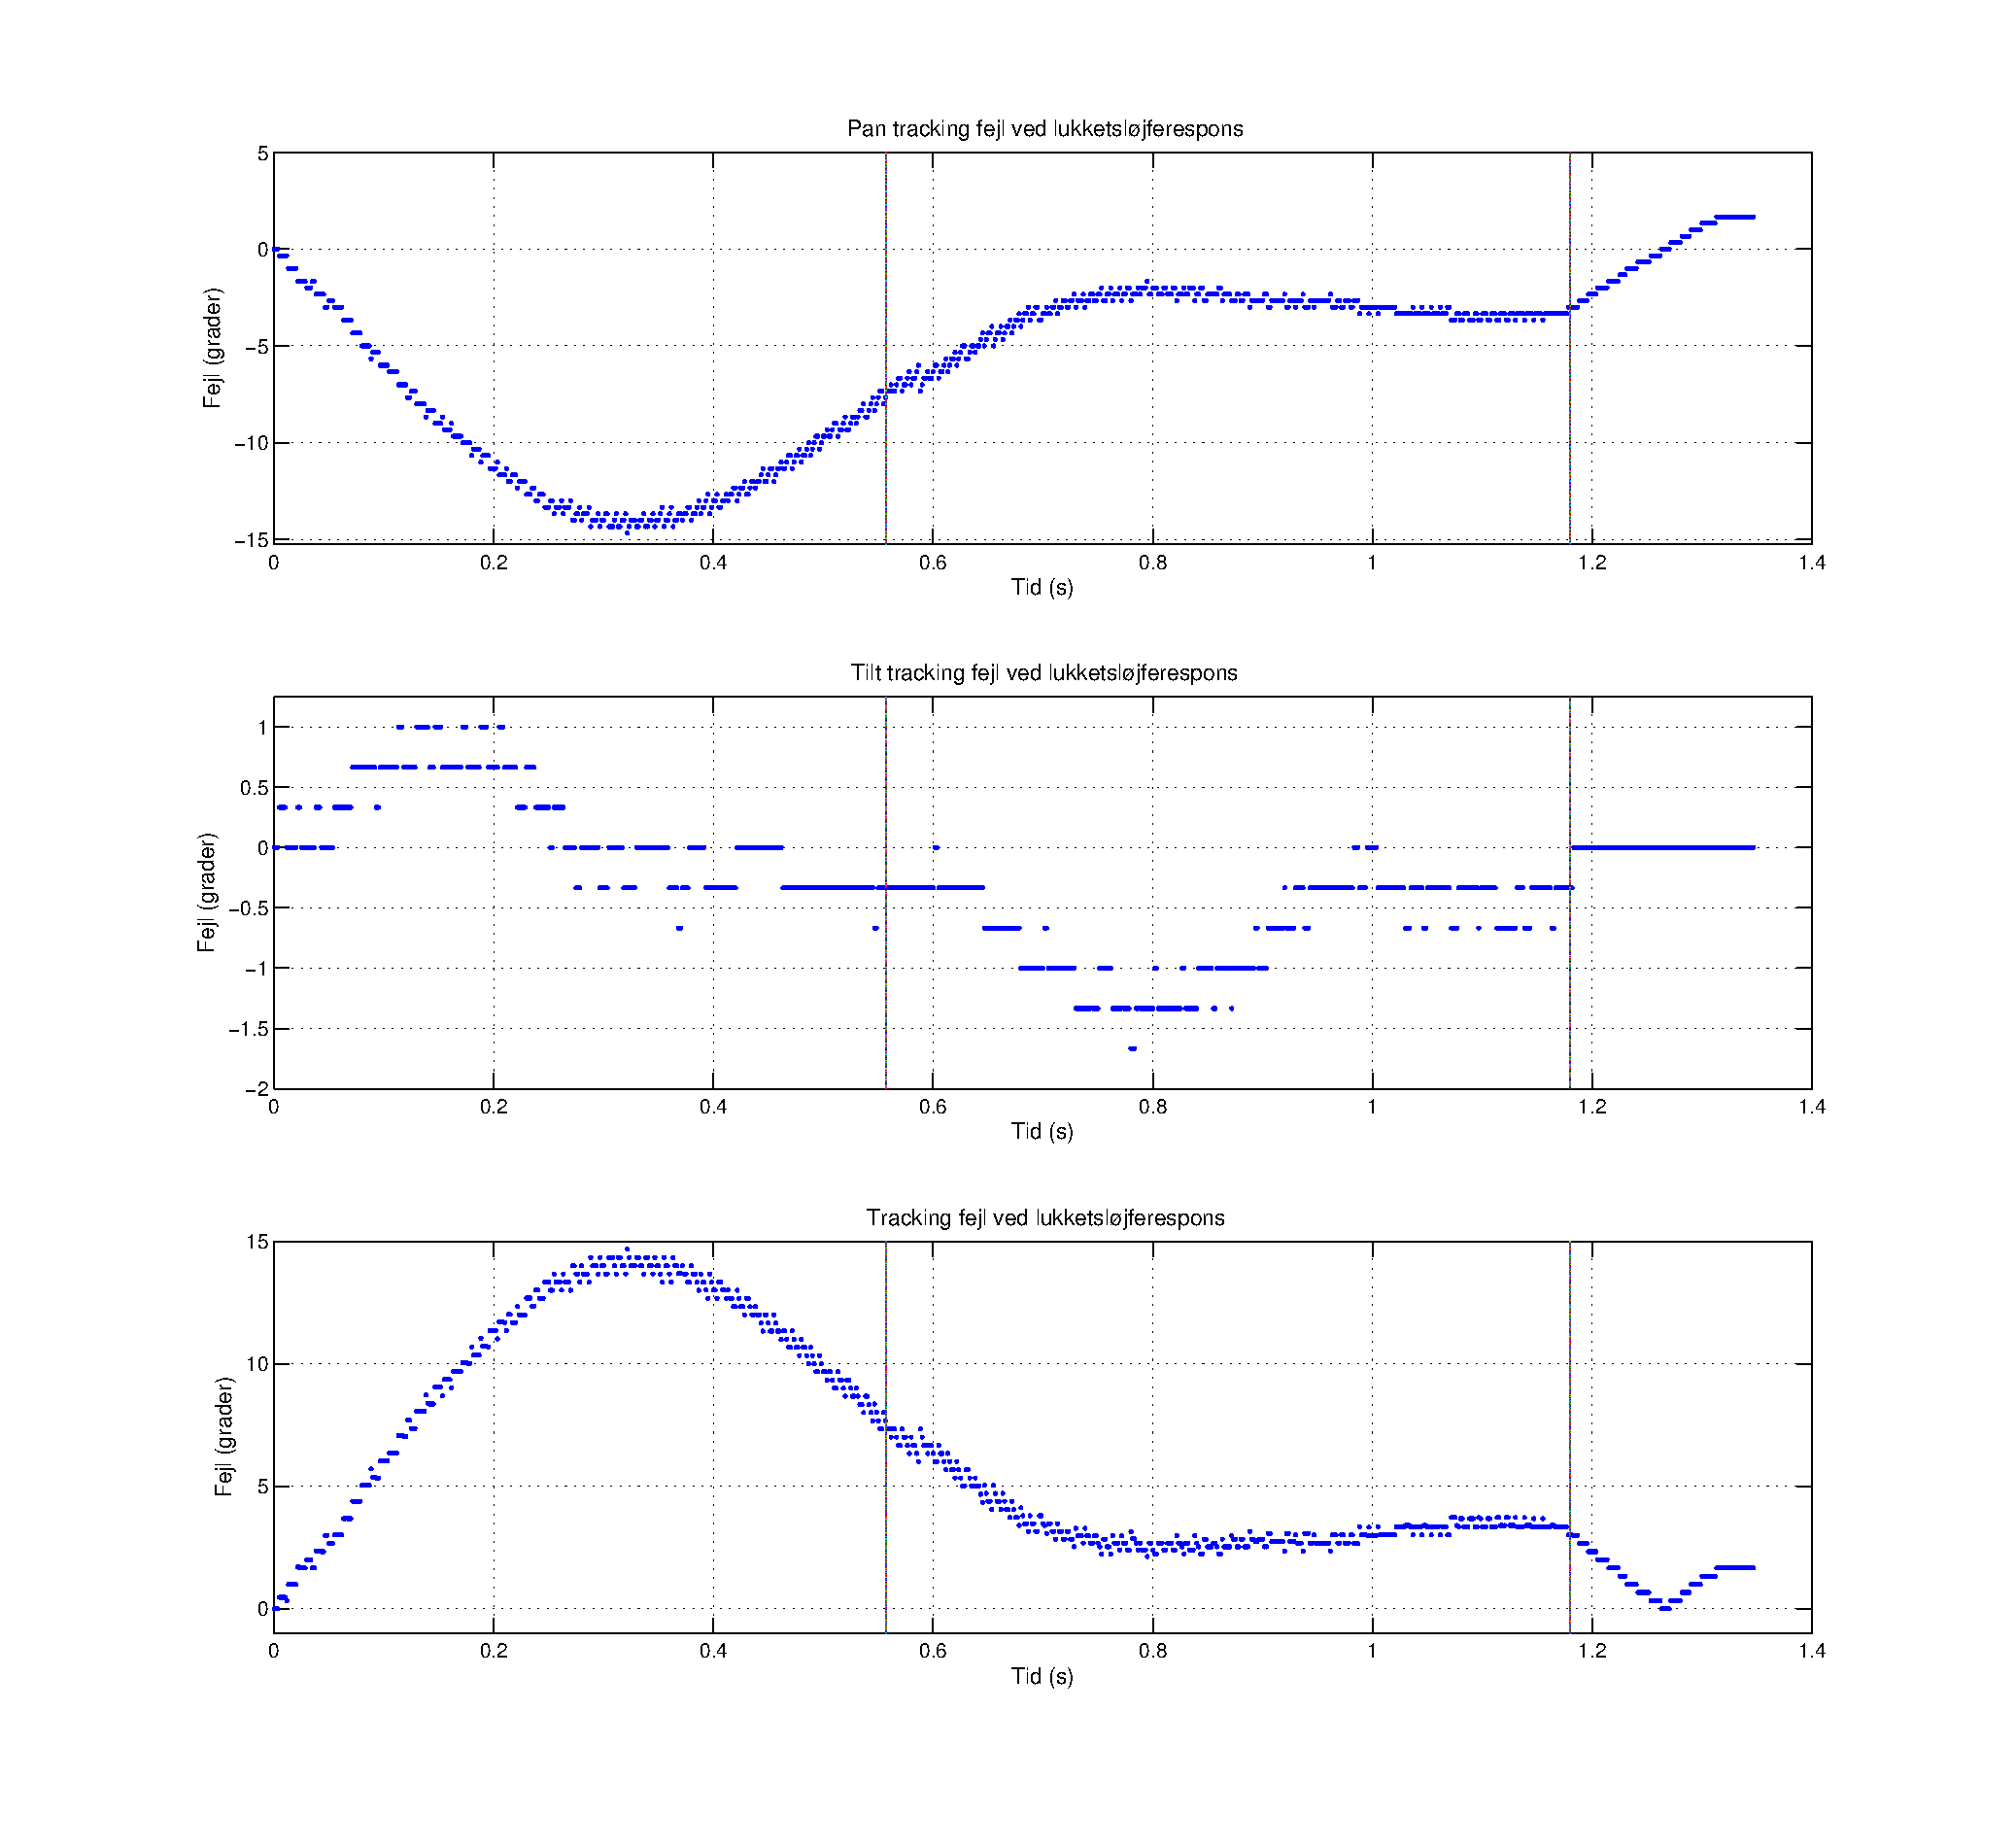
\includegraphics[width=1\textwidth]{./graphics/error_start.eps}
\caption[Regulator koefficienter brugt i test]{Tracking fejl målt i grader for hhv. pan og tilt samt den samlet tracking fejl. Testen tager udgangspunkt i koefficienterne fra  tabel \ref{tb:PID_test14}.} 
\label{fig:PID_test14_plot}
\end{figure}

Det ses tydeligt, at den samlede trackingfejl er langt større end kravet om en 
maksimal trackingfejl på 1.02 \degree.
Det vurderes derfor, at yderligere manuel justering af regulatoren er nødvendig.

\subsection{Manuel justering ift. fysisk PTS}

Ved at ændre på koefficienterne og analysere fejlgraferne justeres performance 
hen mod det ønskede.

Det ses at trackingfejlkravet kan opfyldes med en PI regulator på tilt.
På pan er der behov for en hurtigere reaktion, hvilket medfører et større overshoot. 
For at mindske overshootet vurderes det, at der på pan er behov for en PID 
regulator.

\todo[inline,color=Pink,author=Mikkel]{Ovenstående er meget kvalitativt -  men alternativet er at vi skal have en del grafer, som let kommer til at fylde mange sider.}

\subsubsection{Valg af integratormætning}
Det vælges at sætte integratormætningen til 100 for begge regulatorer betyder, da det vurderes, at der drages
fuld nytte af integratorleddet, da ligning \ref{eq:integratorsaturation} 
overholdes.

\begin{equation}
	K_I \cdot Integrator_{Max} > PWM_{Max}
\label{eq:integratorsaturation} 
\end{equation}

\todo[inline,color=Pink,author=Mikkel]{Måske for kvalitativt. Måske må man ikke bare lave sin egen ligning, men jeg har ikke nogne kilde.}

\subsubsection{Tilføjelse af et D-filter}
Det vurderes at kravene for Pan rammen ikke kunne opnåes vha. en standard PID regulator. 
Det vælges derfor at tilføje et filter til D-leddet. 
Det betyder at D-leddet nu vægter tidligere ændringer i error signalet. 
Filtret reducerer peaks i det differrencierede errorsignal, der skyldes ZoH i upsamplingen (se afsnit \ref{subsec:upsampling}).

Der implementeres et 4. ordens FIR filter. Filtret er designet i fdatool med brug af at Kaiser vindue. Filtrets step og frekvensrespons kan ses på fig. \ref{fig:d_filter_step} hhv. \ref{fig:d_filter_bode}. 

\begin{figure}[h!]
\centering
\subfloat[Steprespins for det implementerede filter.\label{fig:d_filter_step}]{%
	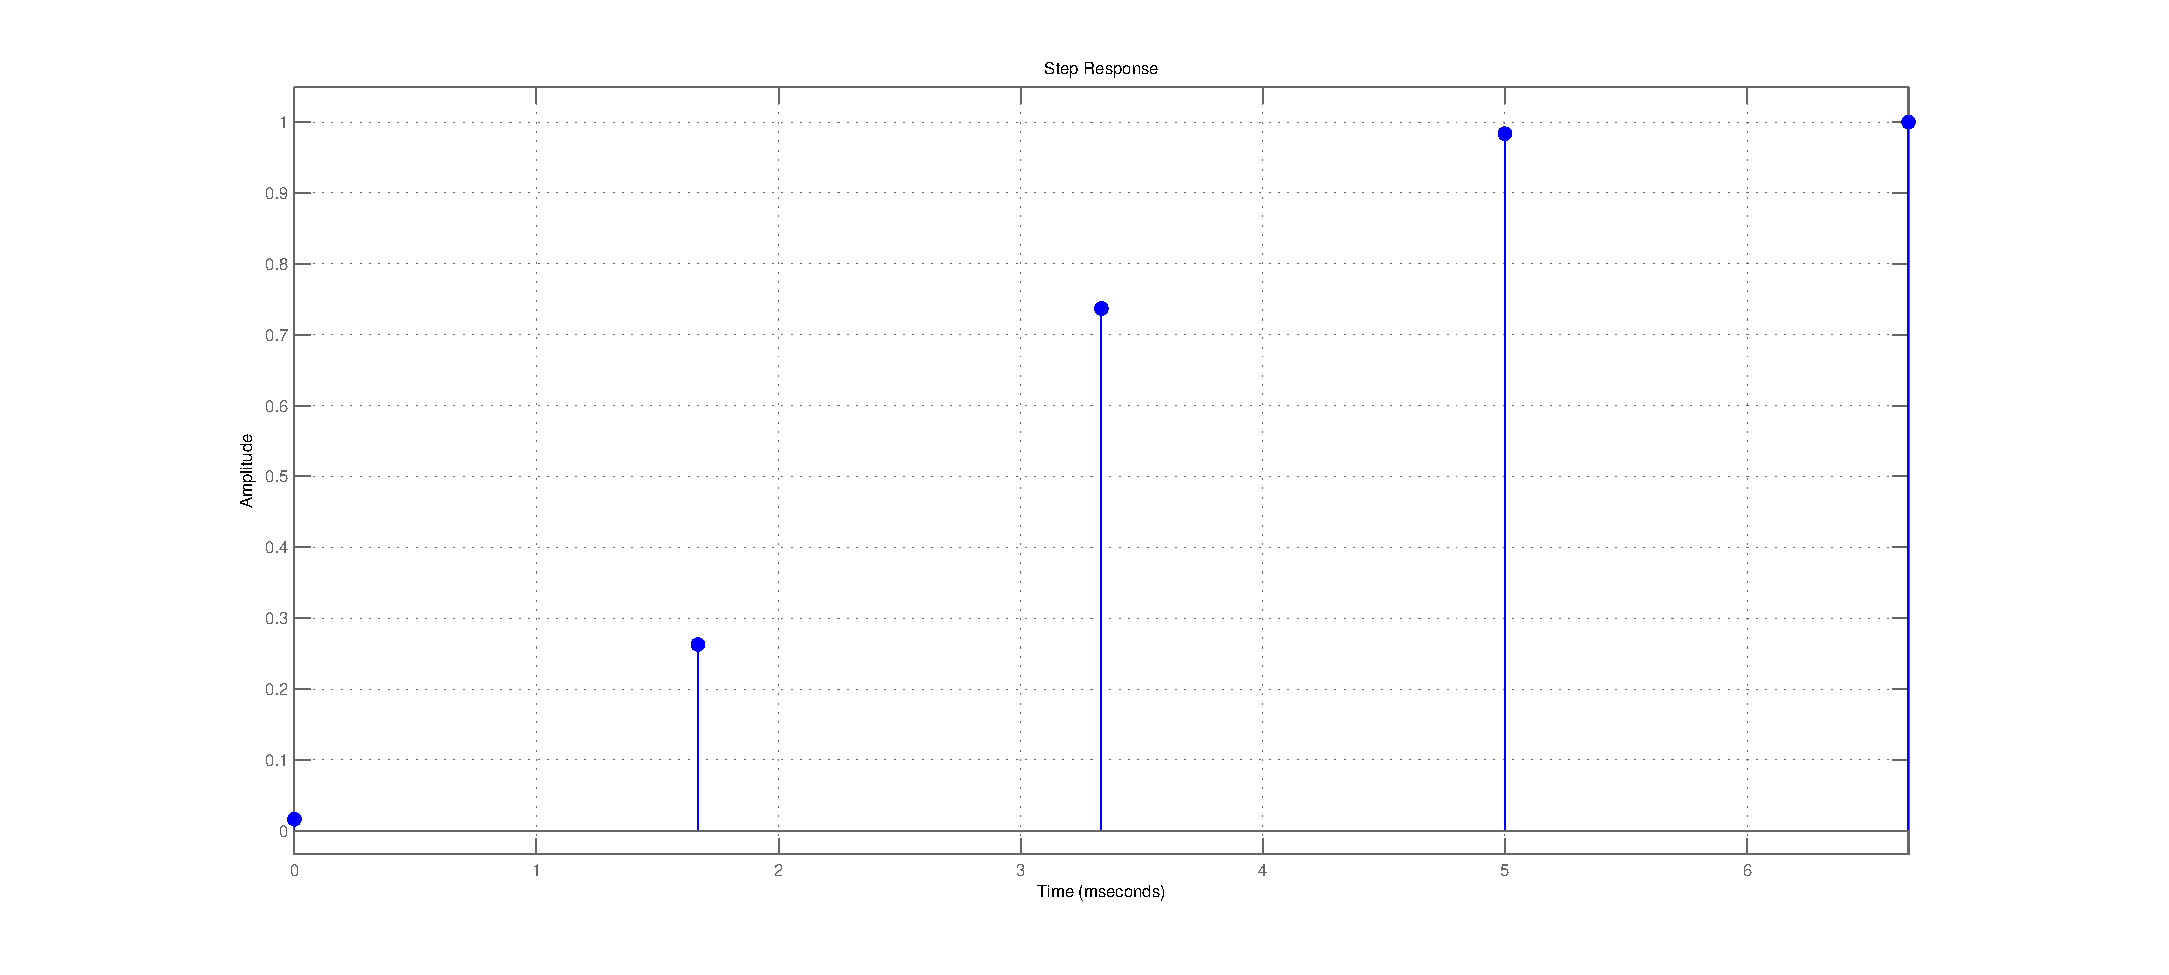
\includegraphics[width=0.7\textwidth]{./graphics/d-filter-step}
}
\subfloat[Frekvensrespons for det implementerede filter.\label{fig:d_filter_bode}]{%
	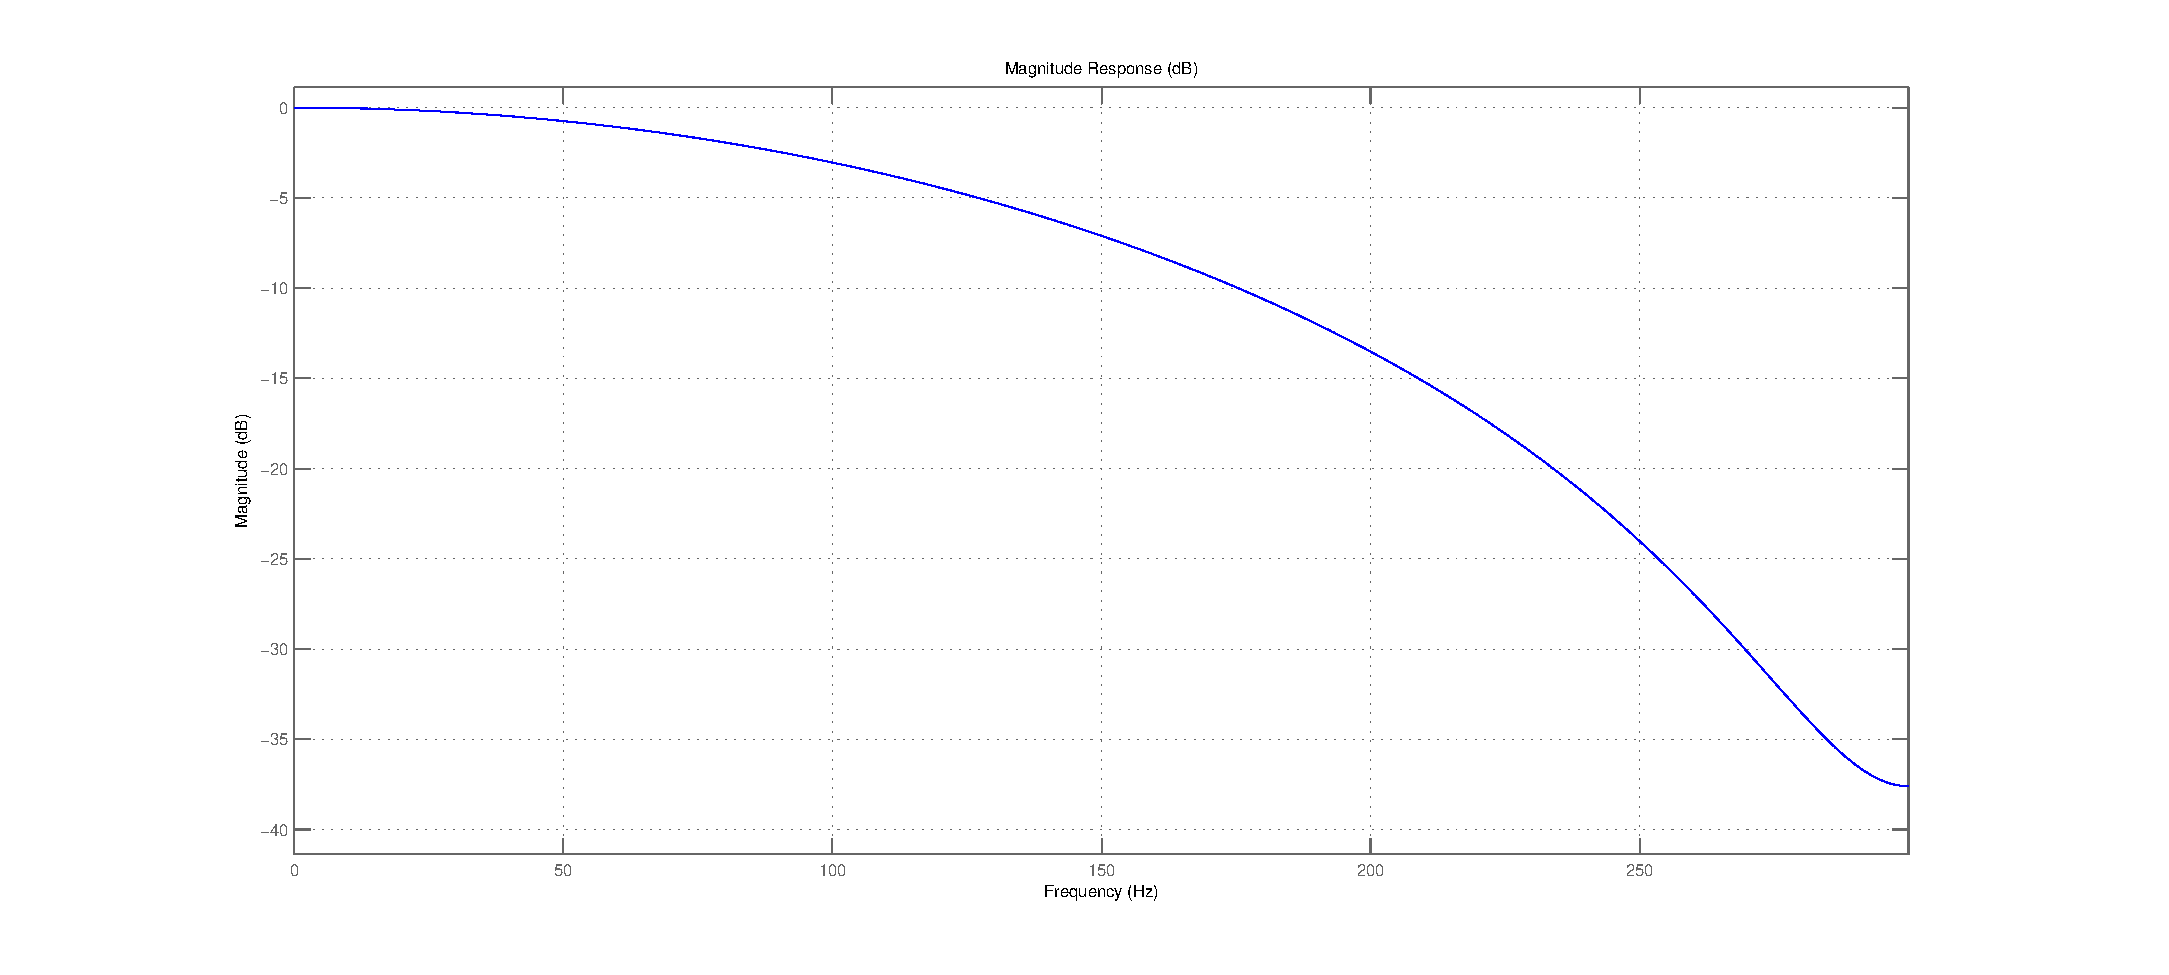
\includegraphics[width=0.7\textwidth]{./graphics/d-filter-bode}
	
}
%\caption[Lerduens parabel i 2D]{Viser parablen af lerduens bane i 2D.}
\label{fig:d_filter}
\end{figure}


%Som det fremgår af figur \ref{fig:PID_test14_plot}, er den samlet tracking fejl XXXXXXXXXXXXXX i 
%forhold til kravene for PTS. Grundet tracking fejlen skal optimeringen af controller koefficienterne
 %foretages manuelt.
%Finjusteringen af controller koefficienterne udføres som en iterativ proces. Optimeringsprocessen 
%er opdelt i to, således der kun foretages ændringer for enten pan eller tilt. 
%Optimerings iterationerne tager udgangspunkt i en grafisk afbildning af tracking fejlen, 
%hvor efter det vurderes hvorledes hver controller koefficient skal øges eller mindskes for at få det ønsket resultat. 
%Der blev foretaget XXXXXXXXXX ilterationer og det lykkes at få en samlet tracking fejl 
%som opfylder kravet, angivet i ligning \ref{eq:ks:trackingerror}.



\subsubsection{Endelig performance}
%For ilteration XXXXXXXXX med controller koefficienterne angivet i tabel \ref{tb:PID_final}, er det 
%lykkedes at opfylde kravet om den samlede tracking fejl som stilles for PTS. 
%Figur \ref{fig:PID_final} viser tracking fejlen for hhv. pan og tilt samt den samlede tracking fejl. 

Efter adskillige test og finjustering af regulatoren, vurderes det at 
koefficienterne i tabel \ref{tb:PID_final} giver den bedst mulige performance 
for PTS. Denne performance ses i \ref{fig:PID_final}. Det ses at trackingfejlen 
holder sig inden for de 1.02$\degree$  pånær ved et par enkelte samples.

\begin{figure}[h!]
\centering
\begin{tabu}{l|[1.25pt]c|c|c}
      & \(K_P\) & \(K_I\) & \(K_D\)\\\tabucline[1.25pt]{-}
Tilt  & 49 & 32.5 & 0\\\hline
Pan   & 80 & 160 & 3.55
\end{tabu}
\captionsetup{type=table}
\caption[Endelige regulatorkoefficienter]{De endelige regulatorkoefficienter.}
\label{tb:PID_final} 
\end{figure}

\begin{figure}[h!]
\centering
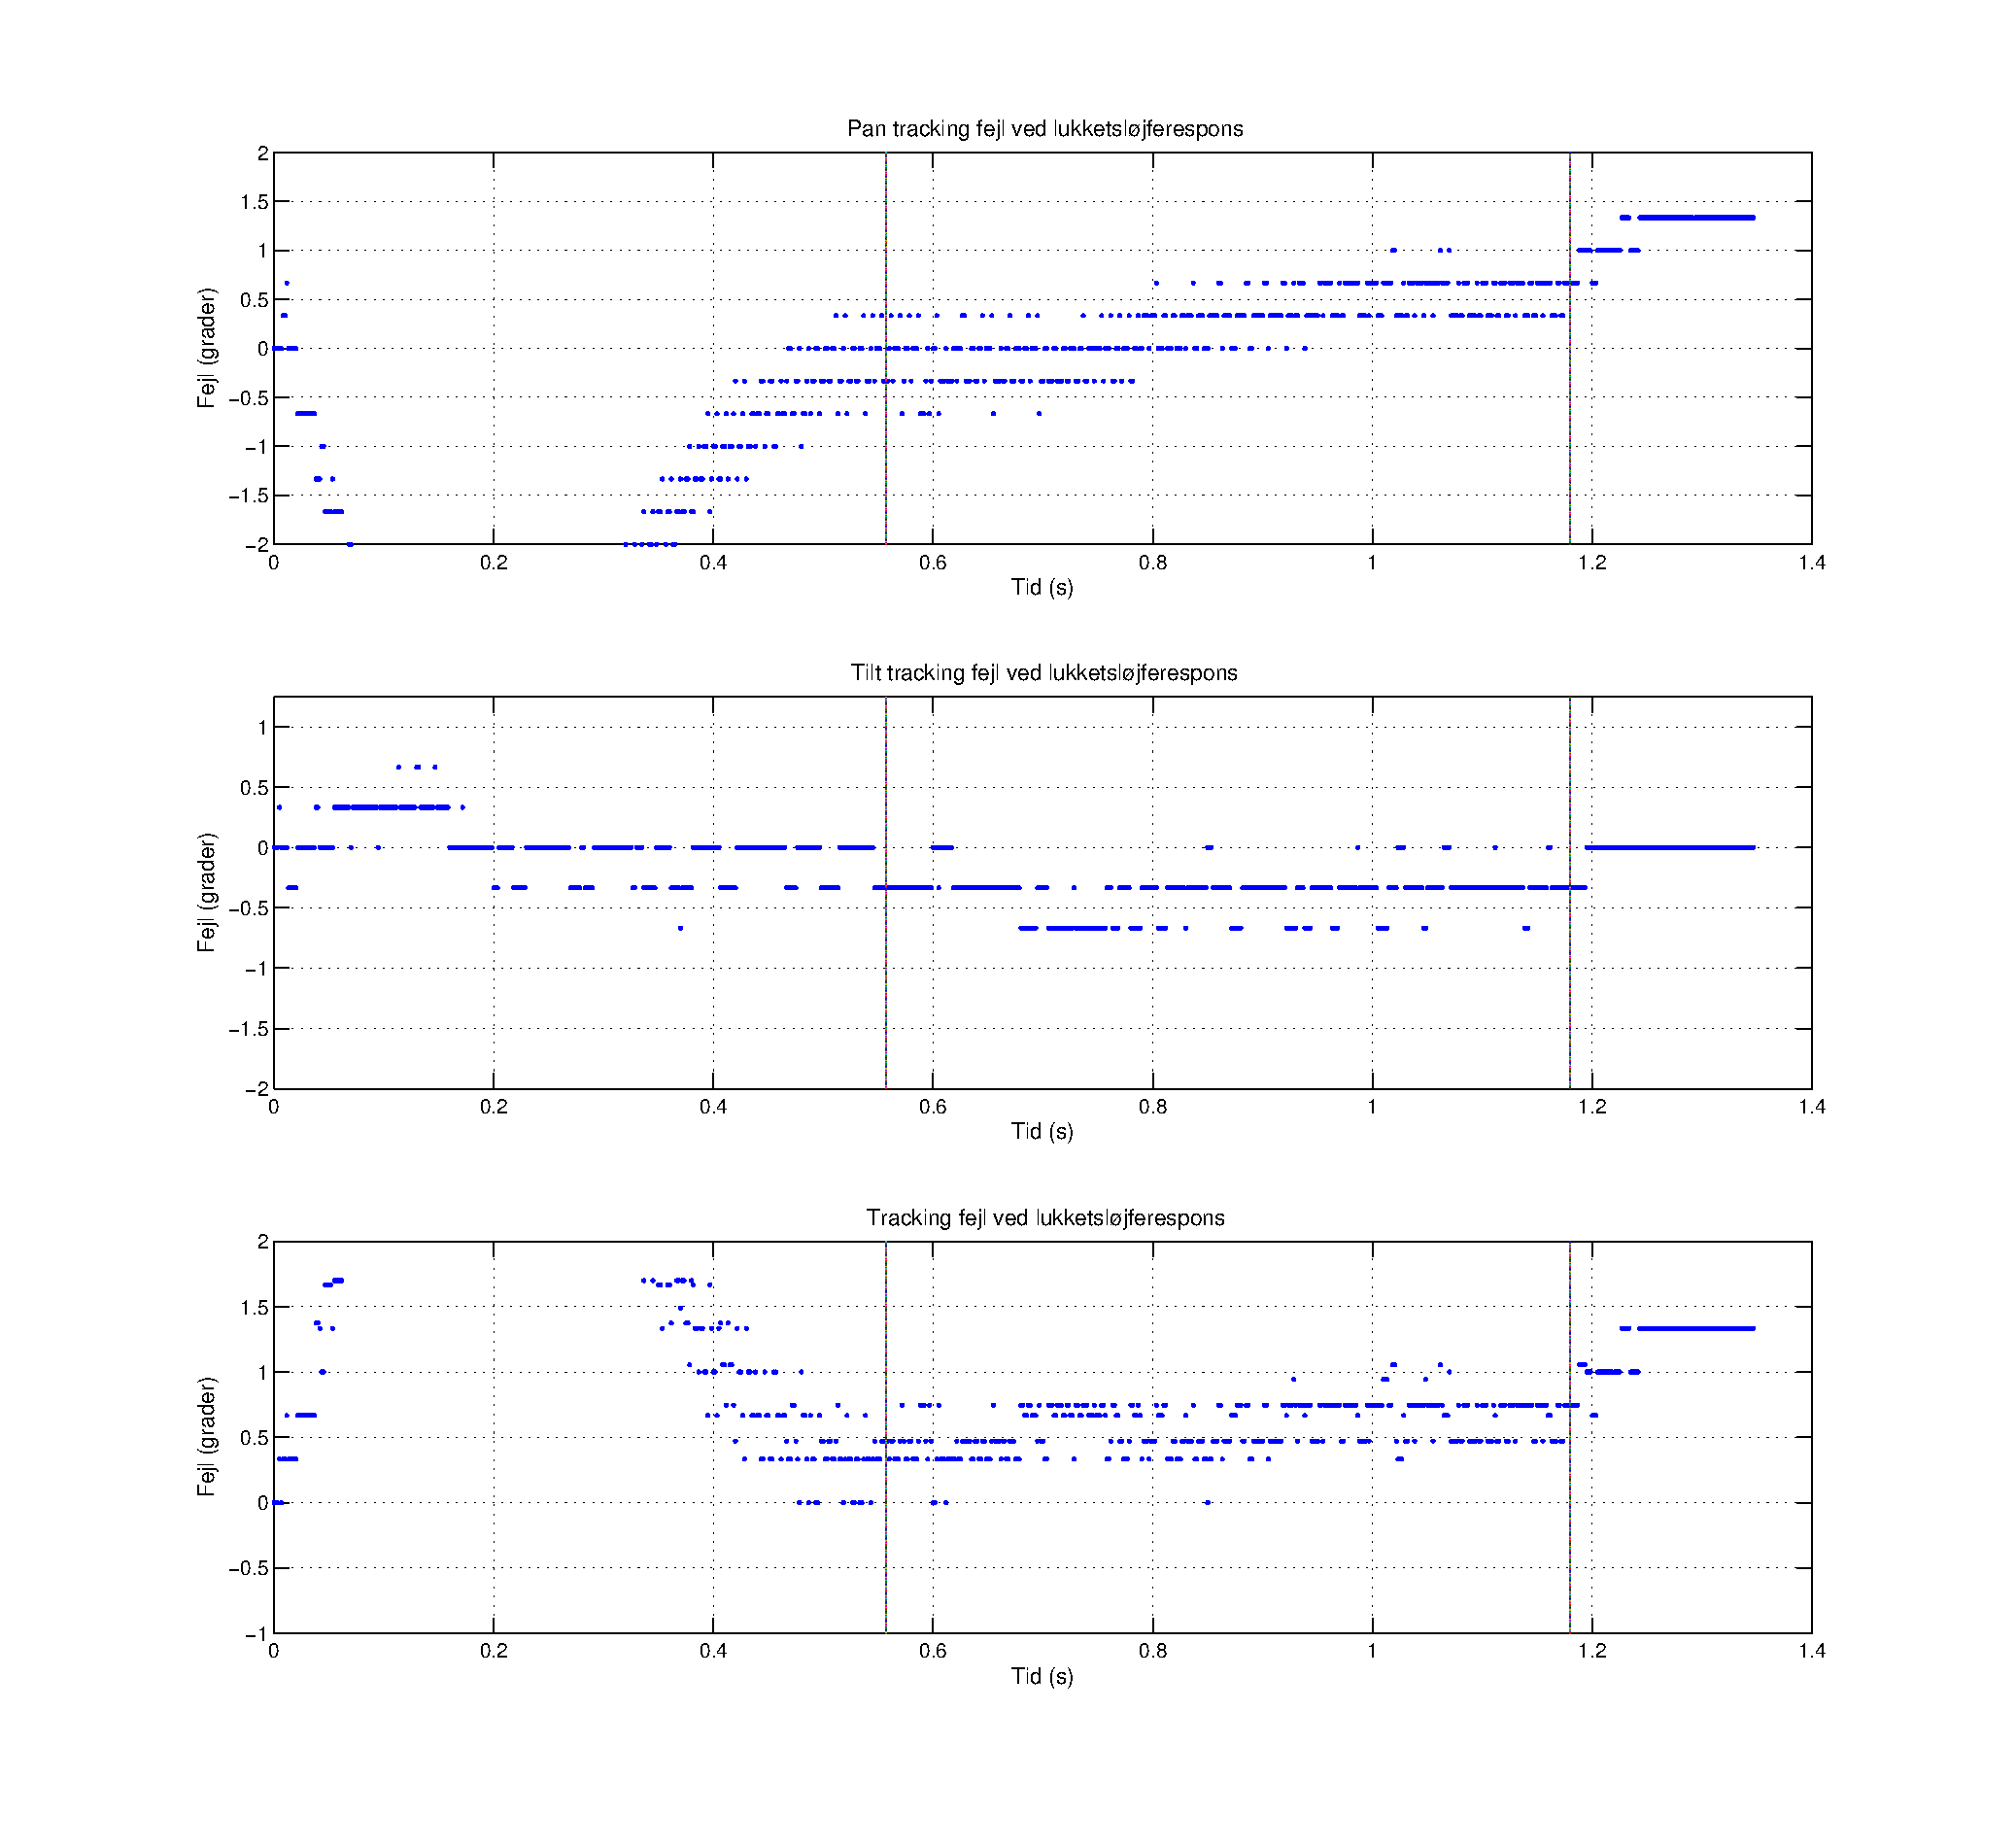
\includegraphics[width=1\textwidth]{./graphics/error_slut.eps}
\caption[Endelig regulator koefficienter]{Tracking fejl målt i grader for hhv. pan og tilt samt den samlet tracking fejl. Testen tager udgangspunkt i koefficienterne fra  tabel \ref{tb:PID_final} og det ses at den samlet tracking fejl opfylder kravet til PTS.} 
\label{fig:PID_final}
\end{figure}

\todo[inline,color=Pink,author=Mikkel]{På begge fejlgrafen bør der stå trackingfejl i stedet for samlet fejl.}

\subsection{Delkonlusion}
Ved trial \& error blev regulatorkoefficienterne justeret til at give den ønskede 
steprespons. Disse koefficienter giver dårlige performance ved PTS. 
Efter yderligere manuel justering med PI regulator og integratormætning på pan og tilt lykkedes 
det ikke at få den ønskede performance på pan. 
Derfor laves en PID regulator med D-filter til pan. Med denne PID regulator til pan og 
PI regulatoren til tilt opnås den ønskede performance. 
Trackingfejlen holdes under kravet på 1.02 \degree pånær ved et par enkelte 
samples.
